\documentclass{beamer}

\usepackage{soul}


\usetheme{Boadilla} 		

\setbeamersize{text margin left=1cm,text margin right=1cm}

% DEFINITON FOOTLINE
% here: empty
\setbeamertemplate{footline}
{%
\begin{beamercolorbox}{}
\end{beamercolorbox}%
}


\usepackage[english]{babel}
\usepackage[latin1]{inputenc}
\usepackage{color}
\usepackage{graphicx}
\graphicspath{{img/}}
\usepackage{setspace}	
%\usepackage[pdftex]{graphicx}

%TABELLEN
\usepackage{array}
%\usepackage{ctable}		%Tabellen mit Fu�oten
\usepackage{multirow}
\usepackage{booktabs}
	% Neue Tabellenbefehle in der array Umgebung
	\renewcommand{\arraystretch}{1.2} % Zeilenabstand
	\newcolumntype{C}[1]{>{\centering\let\\\tabularnewline}p{#1}}
	\newcolumntype{R}[1]{>{\raggedleft\let\\\tabularnewline}p{#1}}
	\newcolumntype{L}[1]{>{\raggedright\let\\\tabularnewline}p{#1}}

\setbeamercovered{transparent}


\title{\'Arboles de Regresi\'on}
\author{Jorge Gallego}
\institute{Inter-American Development Bank}
	
\date{2026}

\begin{document}

%%%%%%%%%%%%%%%%%%%%%%%%%%%%%%%%%%%%%%%%%%%%%%%
\frame{\titlepage}
%%%%%%%%%%%%%%%%%%%%%%%%%%%%%%%%%%%%%%%%%%%%%%%

\frame{
  \frametitle{Introducci\'on}


\begin{itemize}
\item Vimos la esencia de los \'arboles de clasificaci\'on \vspace{0.3cm}

\item Dividir el conjunto de opciones en diferentes subconjuntos por medio de splits en las caracter\'isticas    \vspace{0.3cm}

\item La idea es pasar de grupos heterog\'eneos a conjuntos homog\'eneos\vspace{0.3cm}

\item Al final, la categor\'ia a la que pertenezcan la mayor\'ia de objetos determina la predicci\'on\vspace{0.3cm}

\item Veremos que este m\'etodo tambi\'en sirve para hacer predicci\'on num\'erica\vspace{0.3cm}

\item Por medio de los \textit{\'arboles de regresi\'on} y los \'arboles modelo


\end{itemize}

}


%%%%%%%%%%%%%%%%%%%%%%%%%%%%%%%%%%%%%%%%%%%%%%%

\frame{
  \frametitle{Introducci\'on}


\begin{itemize}

\item Los \'arboles de regresi\'on fueron introducidos en los 1980's con el algoritmo CART (\textit{Classification and Regression Tree}) \vspace{0.3cm}

\item A pesar del nombre, no se usan m\'etodos de regresi\'on \vspace{0.3cm}

\item Las predicciones se basan en el el promedio de los valores de los objetos que quedan en cada hoja\vspace{0.3cm}

\item Luego en lugar de usar la regla de la mayor\'ia (como en clasificaci\'on), promediamos


\end{itemize}

}


%%%%%%%%%%%%%%%%%%%%%%%%%%%%%%%%%%%%%%%%%%%%%%%

\frame{
  \frametitle{Introducci\'on}


\begin{itemize}

\item Los \'arboles modelo (\textit{model trees}) fueron introducidos despu\'es de los \'arboles de regresi\'on \vspace{0.3cm}

\item Se construyen de la misma forma: haciendo \textit{splits} en las variables de inter\'es\vspace{0.3cm}

\item Pero en cada nodo terminal (hoja), se corre un modelo de regresi\'on m\'ultiple usando las observaciones de ese nodo\vspace{0.3cm}

\item Dependiendo del n\'umero de nodos terminales pueden terminar corri\'endose muchos modelos\vspace{0.3cm}

\item Al final, son menos intuitivos pero pueden ser m\'as precisos que los \'arboles de regresi\'on


\end{itemize}

}


%%%%%%%%%%%%%%%%%%%%%%%%%%%%%%%%%%%%%%%%%%%%%%%

\frame{
  \frametitle{Ventajas de estos Modelos}


Las principales ventajas de estos modelos son:\vspace{0.3cm}

\begin{itemize}

\item[1.] Combinan las fortalezas de los \'arboles de decisi\'on para modelar \textit{outcomes} num\'ericos  \vspace{0.3cm}

\item[2.] No se requiere especificar un modelo ex ante\vspace{0.3cm}

\item[3.] La selecci\'on de caracter\'isticas es autom\'atica, luego pueden usarse muchas\vspace{0.3cm}

\item[4.] Se alcanza mejor ajuste que con regresiones para ciertos tipos de datos\vspace{0.3cm}

\item[5.] La intepretaci\'on de los resultados puede ser intuitiva

\end{itemize}

}


%%%%%%%%%%%%%%%%%%%%%%%%%%%%%%%%%%%%%%%%%%%%%%%

\frame{
  \frametitle{Desventajas de estos Modelos}


Las principales desventajas  son:\vspace{0.3cm}

\begin{itemize}

\item[1.] Menos conocidos que la regresi\'on lineal  \vspace{0.3cm}

\item[2.] Se requieren muchos datos de entrenamiento\vspace{0.3cm}

\item[3.] Dif\'icil determinar el efecto neto total de una caracter\'istica sobre el \textit{outcome}\vspace{0.3cm}

\item[4.] \'Arboles muy grandes pueden ser m\'as dif\'iciles de interpretar\vspace{0.3cm}


\end{itemize}

}


%%%%%%%%%%%%%%%%%%%%%%%%%%%%%%%%%%%%%%%%%%%%%%%

\frame{
  \frametitle{\'Arboles vs Regresiones}



\begin{itemize}

\item Para predicci\'on num\'erica el m\'etodo de regresi\'on es mucho m\'as popular  \vspace{0.3cm}

\item Pero en algunos casos los \'arboles de regresi\'on y los modelos de \'arbol son preferibles \vspace{0.3cm}

\item Por ejemplo, cuando hay muchos predictores. O cuando hay no-linealidades \vspace{0.3cm}

\item Adem\'as, con los \'arboles no es necesario imponer muchos de los supuestos sobre la distribuci\'on de los datos



\end{itemize}

}


%%%%%%%%%%%%%%%%%%%%%%%%%%%%%%%%%%%%%%%%%%%%%%%

\frame{
  \frametitle{Medida de Pureza}



\begin{itemize}

\item Vimos que la esencia del m\'etodo  es dividir en caracter\'isticas que nos lleven a grupos m\'as homog\'eneos \vspace{0.3cm}

\item En clasificaci\'on usamos como medida de pureza el \'indice de entrop\'ia \vspace{0.3cm}

\item Pero dicha medida solo puede usarse para outcomes binarios\vspace{0.3cm}

\item ?`Qu\'e medida podemos usar ahora que el outcome es continuo?\vspace{0.3cm}


\end{itemize}

}


%%%%%%%%%%%%%%%%%%%%%%%%%%%%%%%%%%%%%%%%%%%%%%%

\frame{
  \frametitle{Medida de Pureza}



\begin{itemize}

\item Para los \'arboles de regresi\'on usaremos la Reducci\'on en la Desviaci\'on Est\'andar (SDR):

\[
SDR=sd(T)-\sum_i\frac{|T_i|}{|T|}\times sd(T_i)
\]

\item donde $sd(T)$ es la desviaci\'on est\'andar de los valores en el conjunto $T$\vspace{0.3cm}

\item $T_i$ es el conjunto de valores $i$ que resulta de la divisi\'on en una caracter\'istica\vspace{0.3cm}

\item $|T_i|$ es el cardinal del conjunto $T_i$, o el n\'umero de elementos en el conjunto 


\end{itemize}

}


%%%%%%%%%%%%%%%%%%%%%%%%%%%%%%%%%%%%%%%%%%%%%%%

\frame{
  \frametitle{Medida de Pureza}



\begin{itemize}



\item Intuitivamente la f\'ormula mide el cambio en la desviaci\'on est\'andar de los objetos \vspace{0.3cm}

\item Restando a la desviaci\'on del conjunto original, la suma ponderada de las desviaciones de los subconjuntos resultantes\vspace{0.3cm}

\item Como antes, el algoritmo divide en la caracter\'istica que logra el mayor SDR\vspace{0.3cm}

\item Ya que dicha divisi\'on es la que garantiza subconjuntos m\'as homog\'eneos



\end{itemize}

}


%%%%%%%%%%%%%%%%%%%%%%%%%%%%%%%%%%%%%%%%%%%%%%%

\frame{
  \frametitle{Ejemplo}


Consideremos el siguiente ejemplo:

\begin{figure}
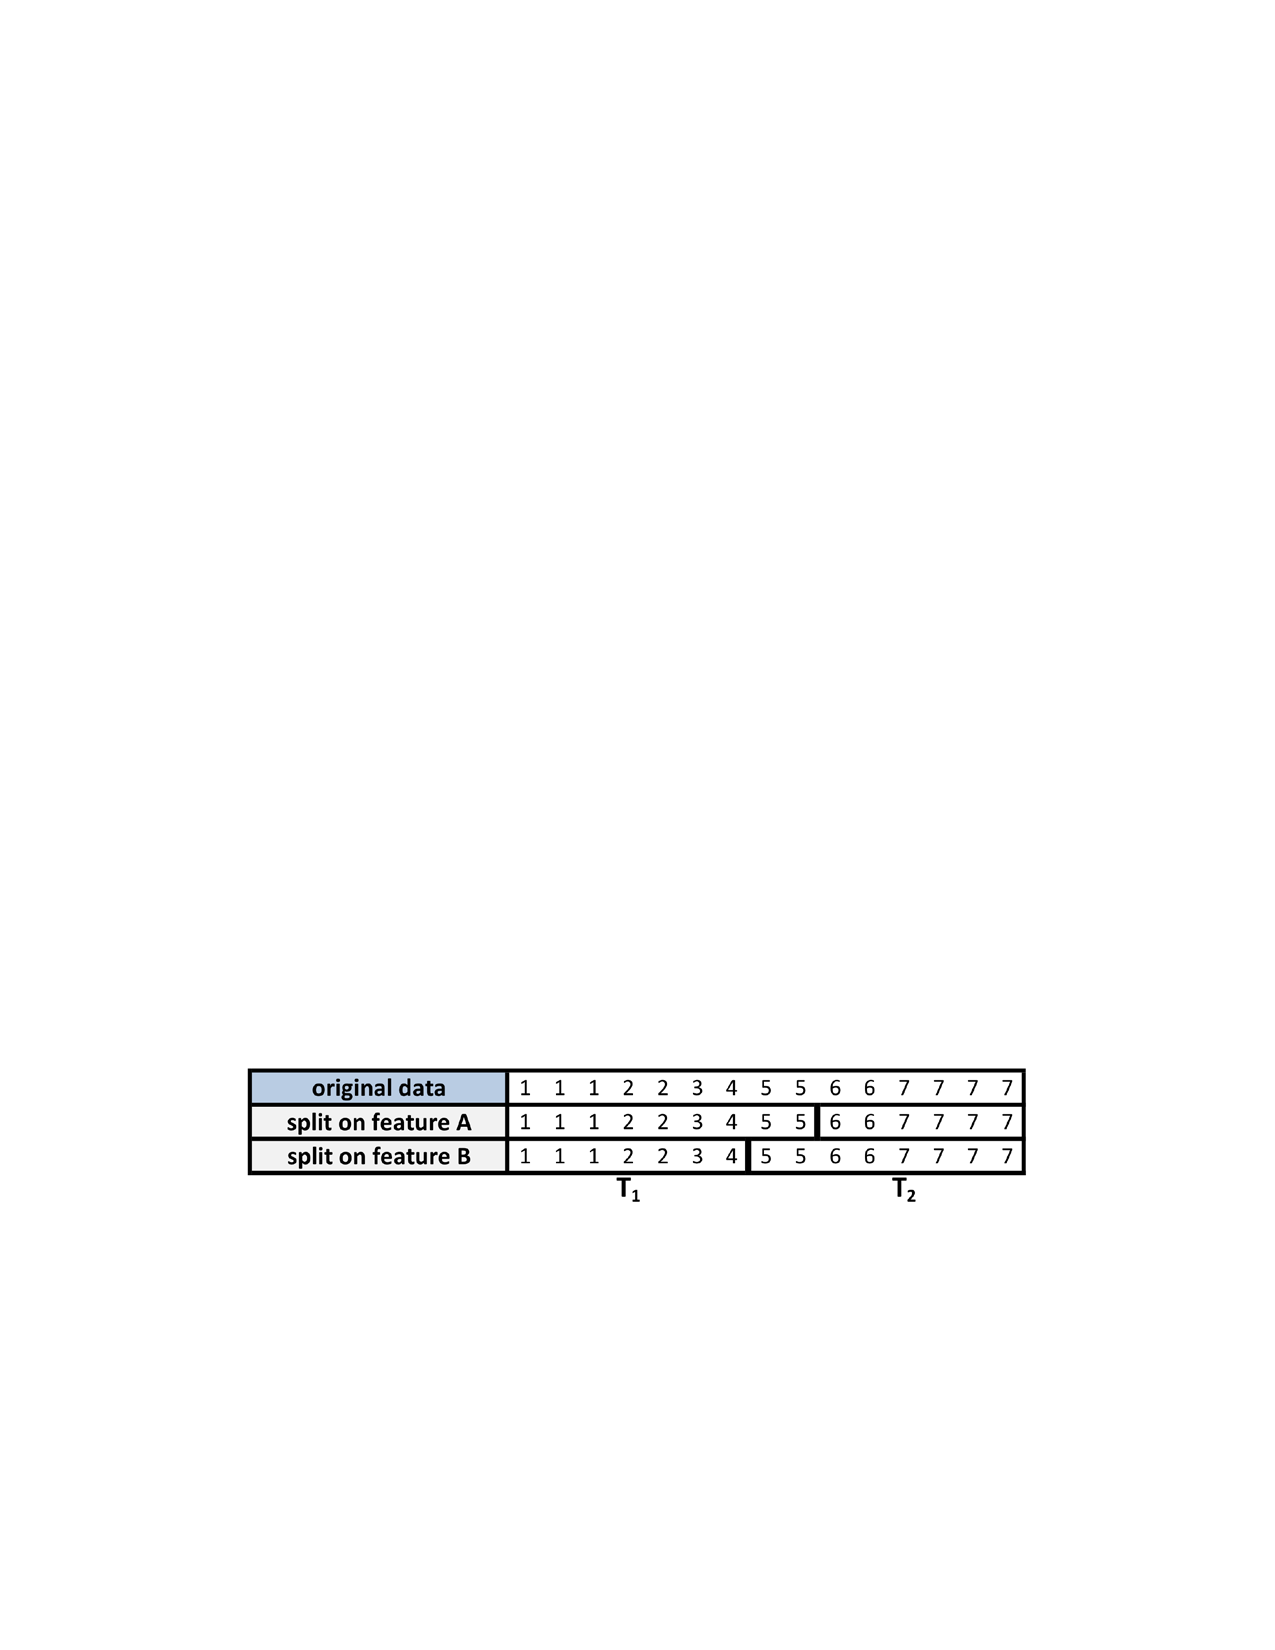
\includegraphics[scale=0.8]{ejemplo}
\end{figure}



}


%%%%%%%%%%%%%%%%%%%%%%%%%%%%%%%%%%%%%%%%%%%%%%%


\frame{
  \frametitle{Ejemplo}



\begin{itemize}


\item La desviaci\'on est\'andar del conjunto original es: $sd(T)=2.404361$ \vspace{0.3cm}

\item La desv. est. ponderada para el split $A$ es: $sd(A)=1.201547$  \vspace{0.3cm}

\item Luego, para el split $A$: $SDR_A=1.202815$ \vspace{0.3cm}

\item La desv. est. ponderada para el split $B$ es: $sd(B)=1.01161$\vspace{0.3cm}

\item Luego, para el split $B$: $SDR_B=1.392751$\vspace{0.3cm}

\item Por tanto, es mejor hacer el split $B$


\end{itemize}

}


%%%%%%%%%%%%%%%%%%%%%%%%%%%%%%%%%%%%%%%%%%%%%%%

\frame{
  \frametitle{Ejemplo}



\begin{itemize}


\item Se hace esto en cada nodo hasta terminar. Qu\'e hacer en cada nodo terminal depende del m\'etodo \vspace{0.3cm}

\item Bajo un \'arbol de regresi\'on, se promedia el outcome para todos los objetos en el nodo\vspace{0.3cm}

\item Esa es la predicci\'on para cualquier objeto nuevo que caiga en ese nodo\vspace{0.3cm}

\item Bajo \'arboles modelo, se corre una regresi\'on y se predice sobre el nuevo outcome



\end{itemize}

}


%%%%%%%%%%%%%%%%%%%%%%%%%%%%%%%%%%%%%%%%%%%%%%%

\frame{
  \frametitle{Ejemplo}



\begin{itemize}


\item En el ejemplo anterior supongamos que hacemos el split en $B$ y se termina el proceso \vspace{0.3cm}

\item Si un objeto cae en $T_1$, bajo \'arbol de regresi\'on la predicci\'on ser\'ia: $mean(T_1)=2$\vspace{0.3cm}

\item Si cae en $T_2$, la predicci\'on ser\'ia: $mean(T_2)=6.25$\vspace{0.3cm}

\item Si se usa un \'arbol modelo, se correr\'ia un regresi\'on en cada nodo terminal \vspace{0.3cm}

\item Y se har\'ia el pron\'ostico con base en dicha regresi\'on



\end{itemize}

}


%%%%%%%%%%%%%%%%%%%%%%%%%%%%%%%%%%%%%%%%%%%%%%%




\end{document}


